\documentclass[UTF8,a4paper,zihao=-4]{ctexart}

\usepackage{geometry}
\usepackage{xcolor}
\usepackage{booktabs}
\usepackage{longtable}
\usepackage{array}
\usepackage{tabularx}
\usepackage{amsmath}
\usepackage{enumitem}
\usepackage{hyperref}
\usepackage{graphicx}
\usepackage{tikz}
\usepackage{pgfplots}
\usepackage{fancyhdr}
\usepackage{titlesec}
\usepackage{caption}
\usepackage{float}

\setCJKmainfont{Noto Serif CJK SC}
\setCJKsansfont{Noto Sans CJK SC}
\setCJKmonofont{Noto Sans Mono CJK SC}
\graphicspath{{figures/}{../../output/imagegen/railway-paper/}}

\usetikzlibrary{arrows.meta,positioning,fit,calc,shapes.geometric,shapes.multipart}
\pgfplotsset{compat=1.18}

\geometry{left=2.5cm,right=2.5cm,top=2.6cm,bottom=2.6cm}
\hypersetup{colorlinks=true,linkcolor=blue!45!black,urlcolor=blue!45!black,citecolor=blue!45!black}
\pagestyle{fancy}
\setlength{\headheight}{15pt}
\fancyhf{}
\fancyhead[L]{面向东南亚铁路运维的多模态智能巡检与风险识别系统}
\fancyhead[R]{DIAI260028GY}
\fancyfoot[C]{\thepage}

\titleformat{\section}{\large\bfseries}{\thesection}{0.8em}{}
\titleformat{\subsection}{\normalsize\bfseries}{\thesubsection}{0.8em}{}
\setlist[itemize]{leftmargin=2em,itemsep=0.2em}
\setlist[enumerate]{leftmargin=2em,itemsep=0.2em}
\renewcommand{\arraystretch}{1.25}

\definecolor{railblue}{HTML}{1F6FAD}
\definecolor{railgreen}{HTML}{198754}
\definecolor{railorange}{HTML}{D97706}
\definecolor{railgray}{HTML}{F2F5F8}
\definecolor{railred}{HTML}{C2410C}
\newcommand{\keynum}[1]{\textcolor{railred}{\bfseries #1}}
\newcommand{\aimark}{（AI辅助生成）}
\newcommand{\realmark}{\textcolor{railred}{\bfseries （真实系统）}}

\tikzset{
  module/.style={draw=railblue!70, fill=railblue!7, rounded corners=3pt, align=center, minimum height=8mm, inner sep=5pt},
  data/.style={draw=railgreen!70, fill=railgreen!8, rounded corners=3pt, align=center, minimum height=8mm, inner sep=5pt},
  risk/.style={draw=railred!75, fill=railred!7, rounded corners=3pt, align=center, minimum height=8mm, inner sep=5pt},
  lang/.style={draw=railorange!80, fill=railorange!8, rounded corners=3pt, align=center, minimum height=8mm, inner sep=5pt},
  arrow/.style={-{Latex[length=2.5mm]}, thick, draw=railblue!75},
  dashedbox/.style={draw=black!25, dashed, rounded corners=4pt, inner sep=8pt}
}

\title{\bfseries 面向东南亚铁路运维的多模态智能巡检与风险识别系统}
\author{工业互联网数智应用解决方案说明书\\[0.6em]
报名编号：DIAI260028GY\\
参赛队员：汤梅婷、李旻晟}
\date{2026年7月}

\begin{document}
\begin{titlepage}
\thispagestyle{empty}
\centering
\vspace*{0.5cm}
{\fontsize{24pt}{34pt}\selectfont\bfseries 面向东南亚铁路运维的多模态智能巡检与风险识别系统\par}
\vspace{0.7cm}
{\Large 工业互联网数智应用解决方案说明书\par}
\vspace{0.8cm}
\includegraphics[width=0.98\textwidth]{01-cover-railway-inspection.png}
\vspace{0.7cm}

\begin{tabular}{rl}
\textbf{核心应用背景：} & 马来西亚东海岸铁路（马东铁/ECRL）\\[0.35em]
\textbf{报名编号：} & DIAI260028GY\\[0.35em]
\textbf{参赛队员：} & 汤梅婷、李旻晟\\
\end{tabular}

\vfill
{\large 2026年7月\par}
\vspace{0.35cm}
{\footnotesize\color{black!60}封面场景图：AI辅助生成\par}
\end{titlepage}

\setcounter{page}{1}
\setcounter{tocdepth}{1}
\begingroup
\small
\tableofcontents
\endgroup
\clearpage

\phantomsection
\addcontentsline{toc}{section}{摘要}
\begin{abstract}
马来西亚东海岸铁路（马东铁，ECRL）正在由工程建设阶段转入运营准备阶段。项目采用中马联合建设、联合运维和本地人才培养模式，大批马来西亚学员赴华接受车站运营、信号、机车驾驶、接触网和车辆维护等专业训练。人员培训解决了技能获取问题，但培训资料、现场视频、风险术语和处置经验仍需要统一的数字化载体，才能支持学员回国后的知识固化、现场复核和远程协同。针对这一需求，本文提出面向东南亚铁路运维的多模态智能巡检与风险识别系统，以马东铁为核心应用背景，构建“数据采集-视频解帧-多模态识别-语义关键词抽取-结构化入库-人工复核”的完整流程。当前原型已实现目标检测、DeepSeek-VL2中文视觉描述、铁路关键词抽取、PostgreSQL数据管理和Web可视化复核，可对轨道、接触网、人员、设备、施工场景和安全风险进行中文语义化组织。本文验证视频均由大疆无人机拍摄，下文统一称为“巡检视频”。原型系统已处理\keynum{24段视频}、\keynum{1716帧图像}，并生成视频级语义名称、帧级描述和风险关键词。该方案形成可检索、可追溯、可审校的中文巡检知识底座，为马东铁及其他东盟铁路项目的本地化运营能力建设提供数智化支撑，并为未来国际化多语种协同保留数据与接口基础。

\textbf{关键词：} 马东铁；东南亚铁路；多模态识别；智能巡检；风险识别；工业互联网
\end{abstract}

\noindent\textcolor{railred}{\bfseries 当前功能边界：}系统现已实现中文视频解帧、图像描述、关键词提取、结构化入库和前端人工复核；双语术语库、双语风险报告及其他东南亚语种均属于后续规划，本文相关架构图表示预留设计，不代表功能已经上线。

\section{项目背景与需求分析}

\subsection{马东铁建设进程与运营转换}

马来西亚东海岸铁路（East Coast Rail Link，ECRL）是连接马来半岛东海岸与西海岸的客货共线铁路。马来西亚交通部资料显示，线路连接吉兰丹州哥打巴鲁与雪兰莪州巴生港，由马来西亚铁路衔接公司（Malaysia Rail Link，MRL）持有项目与资产，中国交通建设股份有限公司（CCCC）承担工程、采购、施工和调试工作\cite{mot-ecrl-overview}。马来西亚交通部2026年2月发布的信息显示，项目全长\keynum{665公里}，截至2026年1月整体进度达到\keynum{91.70\%}，哥打巴鲁至鹅唛综合交通枢纽段计划于2026年底完成，并于2027年1月启动商业运营\cite{mot-ecrl-progress-2026}。

马东铁不是单一施工项目，而是包含工程建设、车辆装备、通信网络、人员培养和长期运营维护的综合铁路系统。2024年中马双方签署联合运维协议，由MRL与CCCC按50:50股比组建合资公司负责运营和维护\cite{ecrl-joint-operation}。这意味着项目重点正在从“能否建成”转向“能否稳定运营、持续维护并形成马来西亚本地能力”，也使巡检知识管理、双语技术资料和现场风险协同成为运营准备期的现实任务。

\begin{table}[H]
\centering
\caption{马东铁运营准备阶段的公开信息与系统需求映射}
\label{tab:ecrl-needs}
\small
\begin{tabularx}{\textwidth}{p{0.22\textwidth}p{0.32\textwidth}X}
\toprule
公开信息 & 项目含义 & 对本方案的需求牵引 \\
\midrule
\keynum{665公里}客货共线铁路，建设进度\keynum{91.70\%} & 由施工期快速进入运营准备期 & 尽快形成可部署、可扩展的数字运维底座 \\
MRL与CCCC联合运维 & 中外团队长期共同承担运营维护 & 需要统一术语、双语记录和跨组织复核流程 \\
2025年计划\keynum{210名}学员赴柳州培训 & 岗位多、批次多、培训周期长 & 需要沉淀课程、案例、现场视频和岗位知识 \\
覆盖信号、司机、接触网、车辆维护等岗位 & 专业边界多且风险规则不同 & 需要按专业组织术语、风险标签和权限 \\
面向东盟推进职业教育与数字资源共享 & 马东铁经验具有区域复制潜力 & 预留英语和东南亚本地语种扩展接口 \\
\bottomrule
\end{tabularx}
\end{table}

\subsection{赴华培训与本地运维能力建设}

马东铁已形成较大规模的本地人才培养体系。早期PLKI-ECRL工业技能培训计划由MRL、CCCC、中国高校和马来西亚教育培训机构共同实施，目标覆盖铁路建设和运营人才\cite{ndrc-ecrl-training}。进入运营维护准备阶段后，马来西亚交通部长在2025年PLKI-ECRL O\&M项目讲话中提出，运营维护阶段计划总体培养\keynum{3200人}；2025年安排\keynum{210名}马来西亚学员赴柳州接受一年强化培训，首批102人分阶段启程，岗位包括车站助理、信号技术员、机车副司机、接触网技术员以及电力机车和动车组维护技术员\cite{mot-plki-2025}。马方同时明确，本地能力建设的目标是减少长期依赖外部专家，而不是形成新的技术依赖。

大量人员赴华培训说明马方对中国铁路建设、装备和职业教育能力具有现实认可，也说明知识转移任务已经从少数专家交流转向多岗位、规模化和长期化的人才体系。2025年中马联合声明将马东铁、铁路运输合作、职业教育、数字教育、人工智能和技术转移并列为重点合作领域，并以相互信任、互利和共同商定为合作原则\cite{china-malaysia-joint-statement}。因此，正式方案使用“技术认可与能力共建”比“技术依赖”更准确，也更符合马方强调本地化运营的政策目标。

\subsection{培训之后的数字资料与运维平台缺口}

现有公开资料充分证明培训、岗位认证和联合运维正在推进，但并未表明培训资料、现场巡检视频、双语术语、风险案例和人工复核记录已经被统一纳入一个可持续的数字知识平台。由此不能简单断言马东铁“没有运维系统”，但可以识别出一个明确的系统建设空间：培训解决“人会不会”，数智平台解决“知识能否持续沉淀、现场问题能否快速复核、不同语言团队能否形成一致记录”。

无人机、移动终端、轨旁摄像头和车载巡检设备能够以较低成本采集大量铁路现场图像与视频。然而，原始视频并不等同于可直接使用的运维知识。人工回看视频不仅耗时，而且难以保证风险识别的一致性；同时，巡检视频中的“接触网、轨道、人员、设备、施工、积水、标识牌、安全风险”等语义要素如果不能被结构化保存，就难以支持后续检索、复核、培训和多语言报告生成。

\begin{figure}[H]
\centering
\includegraphics[width=0.96\textwidth]{05-bilingual-collaboration.png}
\caption{中马铁路运维人员共享巡检结果的概念场景\aimark}
\label{fig:ecrl-collaboration}
\end{figure}

\subsection{中国铁路技术合作趋势与本方案定位}

中国铁路技术国际合作正在从单一工程承包，逐步扩展为“工程建设、装备供应、技术标准、人员培训、联合运维和数字平台”的组合式能力输出。中国与东盟2026-2030行动计划提出加强职业技术教育机构交流、知识分享、技能发展和优质数字教育资源共建共享\cite{asean-china-action-plan}；来自东盟多国的铁路技术人员也在中国参加轨道交通标准和人工智能专题培训，并表达继续开展标准化合作的意愿\cite{asean-rail-training}。这些事实体现的是对中国工程经验的认可和共同建设本地能力的需求，而不是单向依赖。

本文关注的问题不是单一目标检测算法的性能提升，而是构建一个可服务马东铁运营准备和东盟铁路能力建设的可部署系统，使多源巡检数据能够被自动解帧、识别、描述、入库和展示，并与培训资料、铁路术语和风险案例形成联系。系统既适配当前中文巡检语义，也预留中英双语及东南亚多语种扩展能力，从而服务中方工程师、本地技术人员和管理部门的跨语言协同。

本文主要贡献如下：
\begin{enumerate}
  \item 提出面向东南亚铁路运维的多模态智能巡检系统架构，覆盖数据采集、视频解帧、多模态识别、语义关键词抽取、数据管理和前端展示。
  \item 设计铁路巡检语义标签与风险关键词体系，将视觉语言模型生成的自然语言描述转化为视频级和帧级结构化记录。
  \item 预留多语种铁路知识服务架构，为中英双语展示及泰语、老挝语、越南语、印尼语等东南亚语种扩展提供系统接口。
  \item 基于真实巡检视频进行应用验证，完成\keynum{24段视频}、\keynum{1716帧图像}的处理、入库与可视化浏览。
\end{enumerate}

\noindent\textbf{图示说明：}封面场景图与图1标注为“AI辅助生成”，仅用于表达应用构想；红色\realmark 表示来自实际运行平台或真实视频拍摄数据；其余流程图、数据模型图和知识架构图均依据当前系统代码与方案设计绘制。

\subsection{典型场景与核心需求}

\subsubsection{应用场景与痛点}

东南亚铁路运维场景既包含新建线路施工期的安全监管，也包含运营期的设备巡检和故障预防。巡检对象覆盖轨道、接触网、信号设备、线路周边环境、施工人员、作业车辆和安全标识等。图\ref{fig:scenario}给出了本文系统面向的典型场景。

\begin{figure}[H]
\centering
\begin{tikzpicture}[node distance=9mm and 12mm, font=\small]
  \node[data] (uav) {无人机巡检\\高空视频};
  \node[data, below=of uav] (mobile) {移动终端\\现场图片};
  \node[data, below=of mobile] (camera) {轨旁摄像头\\固定视角};
  \node[data, below=of camera] (vehicle) {车载巡检\\连续视频};

  \node[module, right=24mm of mobile, minimum width=35mm, minimum height=34mm] (platform) {多模态智能\\巡检平台};

  \node[module, right=24mm of platform, yshift=18mm] (detect) {目标识别\\轨道/设备/人员};
  \node[module, right=24mm of platform] (risk) {风险识别\\施工/积水/侵限};
  \node[lang, right=24mm of platform, yshift=-18mm] (report) {双语报告（规划）\\跨语言协同};

  \draw[arrow] (uav.east) -- (platform.west);
  \draw[arrow] (mobile.east) -- (platform.west);
  \draw[arrow] (camera.east) -- (platform.west);
  \draw[arrow] (vehicle.east) -- (platform.west);
  \draw[arrow] (platform.east) -- (detect.west);
  \draw[arrow] (platform.east) -- (risk.west);
  \draw[arrow] (platform.east) -- (report.west);

  \node[dashedbox, fit=(uav)(mobile)(camera)(vehicle), label=above:多源数据采集] {};
  \node[dashedbox, fit=(detect)(risk)(report), label=above:运维应用输出] {};
\end{tikzpicture}
\caption{东南亚铁路多模态智能巡检应用场景}
\label{fig:scenario}
\end{figure}

该场景存在四类核心痛点：第一，数据规模大，巡检视频难以人工逐帧分析；第二，风险类型多，单一检测模型难以覆盖复杂场景；第三，语言协同复杂，需要将视觉结果转化为可翻译、可复核的术语化表达；第四，巡检结果需要长期积累，必须以数据库方式保存批次、视频、帧和风险描述。

\subsubsection{多源数据采集要求}

系统不应仅面向单一视频文件，而应面向多源铁路巡检数据。图\ref{fig:data-source}展示了本文设计的数据采集架构。视频、图像、文本记录和术语库共同构成多模态数据底座，其中视频和图像用于当前中文视觉识别，文本和术语库为风险解释及后续多语种生成提供数据基础。

\begin{figure}[H]
\centering
\includegraphics[width=0.96\textwidth]{02-multisource-data-collection.png}
\caption{面向马东铁的多源巡检数据采集概念图}
\label{fig:data-source}
\end{figure}

\section{总体方案设计}

本文系统采用分层架构，如图\ref{fig:architecture}所示。系统自下而上分为数据采集层、数据预处理层、多模态识别层、知识与语言服务层、数据管理层和应用展示层。该架构既覆盖当前已经实现的视频解帧与中文描述功能，也为后续双语和多语种服务提供扩展位置。

\begin{figure}[H]
\centering
\begin{tikzpicture}
  \node[anchor=south west,inner sep=0] (archimg) at (0,0)
    {\includegraphics[width=0.96\textwidth]{03-multimodal-system-architecture.png}};
  \foreach \pos/\txt in {0.083/数据采集,0.25/视频预处理,0.417/多模态识别,0.583/双语服务（预留）,0.75/结构化数据,0.917/人工复核应用} {
    \node[font=\scriptsize\bfseries,text width=22mm,align=center,yshift=19.5mm]
      at ($(archimg.south west)!\pos!(archimg.south east)$) {\txt};
  }
\end{tikzpicture}
\caption{多模态智能巡检系统总体架构}
\label{fig:architecture}
\end{figure}

该架构的关键特点在于将“识别结果”进一步提升为“可管理的巡检知识”。视觉模型负责从图像中提取对象与语义，知识层负责将描述归一化为铁路术语和风险类别，数据库负责保存完整处理链路，前端负责将视频、帧、关键词和描述组织为可复核界面。

\section{关键技术与创新设计}

\subsection{视频解帧与时序索引}

巡检视频首先按照固定时间间隔进行抽帧。本文当前系统采用约每秒一帧的策略，保存帧号、时间戳、帧图片路径和视频来源信息。该方式在计算成本和信息覆盖之间取得平衡，适合对无人机巡检视频进行快速语义化处理。

\begin{figure}[H]
\centering
\begin{tikzpicture}[node distance=10mm and 11mm, font=\small]
  \node[data] (video) {输入视频};
  \node[module, right=of video] (frame) {按时间间隔\\抽取关键帧};
  \node[module, right=of frame] (detect) {目标检测\\YOLO};
  \node[module, right=of detect] (caption) {视觉语言描述\\DeepSeek-VL2};
  \node[lang, below=of caption] (keyword) {关键词抽取\\铁路语义标签};
  \node[risk, left=of keyword] (risk) {风险标签\\施工/人员/设备};
  \node[module, left=of risk] (db) {结构化入库};
  \node[module, left=of db] (web) {前端浏览\\检索复核};

  \draw[arrow] (video) -- (frame);
  \draw[arrow] (frame) -- (detect);
  \draw[arrow] (detect) -- (caption);
  \draw[arrow] (caption) -- (keyword);
  \draw[arrow] (keyword) -- (risk);
  \draw[arrow] (risk) -- (db);
  \draw[arrow] (db) -- (web);
\end{tikzpicture}
\caption{视频帧多模态识别流程}
\label{fig:pipeline}
\end{figure}

\subsection{视觉语言描述}

目标检测模型适合识别边界明确的对象，但铁路巡检场景中还存在大量难以用单一检测框表示的语义信息，例如湿滑地面、施工区域、设备环境、标识牌含义和周边植被。因此，本文引入视觉语言模型对关键帧生成自然语言描述。系统提示词围绕“铁路目标、人员、车辆、轨道、设备、施工场景和安全风险”设计，使生成结果更贴近运维语义。

\subsection{铁路关键词与风险标签抽取}

系统从帧描述文本中抽取视频级关键词，当前关键词体系包括接触网、轨道、人员、设备、车辆、施工、安全风险、标识牌、站场、雨天地面、植被和桥梁等。关键词抽取先采用规则匹配和同义词归一化方式实现，后续可扩展为多标签分类模型或大模型结构化抽取。图\ref{fig:keyword}展示了关键词归一化过程。

\begin{figure}[H]
\centering
\resizebox{0.96\textwidth}{!}{%
\begin{tikzpicture}[node distance=9mm and 8mm, font=\small]
  \node[data, minimum width=36mm] (desc) {帧级中文描述};
  \node[module, right=of desc, minimum width=34mm] (match) {同义词匹配\\术语归一化};
  \node[lang, right=of match, minimum width=34mm] (kw) {关键词集合};
  \node[risk, right=of kw, minimum width=34mm] (risk) {风险类别};

  \node[data, below=of match, xshift=-12mm] (a1) {供电线路/电线杆\\$\rightarrow$ 接触网};
  \node[data, below=of kw] (a2) {工人/作业人员\\$\rightarrow$ 人员};
  \node[data, below=of risk, xshift=-8mm] (a3) {警示/危险/障碍\\$\rightarrow$ 安全风险};

  \draw[arrow] (desc) -- (match);
  \draw[arrow] (match) -- (kw);
  \draw[arrow] (kw) -- (risk);
  \draw[arrow] (a1) -- (match);
  \draw[arrow] (a2) -- (kw);
  \draw[arrow] (a3) -- (risk);
\end{tikzpicture}}
\caption{铁路语义关键词归一化与风险标签抽取}
\label{fig:keyword}
\end{figure}

\subsection{国际化多语种知识服务预留设计}

东南亚铁路运维涉及多语言协作。当前系统仅提供中文描述和中文关键词，尚未实现双语切换、多语种风险报告或本地语种输出。为避免后续在识别链路中重复改造，本文先在架构和数据接口层预留国际化知识服务位置。图\ref{fig:language}给出规划中的知识服务架构，该图表示未来建设目标，而非当前已上线功能。

\begin{figure}[H]
\centering
\resizebox{0.96\textwidth}{!}{%
\begin{tikzpicture}[node distance=8mm and 9mm, font=\small]
  \node[data] (vision) {视觉识别结果};
  \node[data, below=of vision] (caption) {图像描述文本};
  \node[data, below=of caption] (keywords) {铁路关键词};
  \node[module, right=22mm of caption, minimum width=36mm] (norm) {铁路术语\\标准化};

  \node[lang, right=22mm of norm, yshift=18mm] (zh) {中文术语库};
  \node[lang, right=22mm of norm, yshift=6mm] (en) {英文术语库};
  \node[lang, right=22mm of norm, yshift=-6mm] (thai) {泰语/老挝语\\扩展术语库};
  \node[lang, right=22mm of norm, yshift=-18mm] (sea) {越南语/印尼语\\扩展术语库};

  \node[risk, right=28mm of en, yshift=-7mm, minimum width=34mm] (output) {多语种风险表达\\报告/前端/培训};

  \draw[arrow] (vision.east) -- (norm.west);
  \draw[arrow] (caption.east) -- (norm.west);
  \draw[arrow] (keywords.east) -- (norm.west);
  \draw[arrow] (norm) -- (zh);
  \draw[arrow] (norm) -- (en);
  \draw[arrow] (norm) -- (thai);
  \draw[arrow] (norm) -- (sea);
  \draw[arrow] (zh.east) -- (output.west);
  \draw[arrow] (en.east) -- (output.west);
  \draw[arrow] (thai.east) -- (output.west);
  \draw[arrow] (sea.east) -- (output.west);
\end{tikzpicture}}
\caption{面向东南亚铁路的双语与多语种知识服务规划架构}
\label{fig:language}
\end{figure}

后续双语服务的关键不是简单机器翻译，而是铁路术语一致性。比如“接触网、轨道、施工人员、安全风险、设备箱、警示牌”等需要通过术语库进行标准化映射，避免不同语言版本中出现概念漂移。计划采用“中文描述-术语标准化-英文表达-人工审校-本地语种扩展”的分阶段策略：先建设中英及马来语核心术语库和报告模板，再按实际项目需要扩展泰语、老挝语、越南语和印尼语。

\section{系统实现与验证}

\subsection{数据库设计}

为了支持巡检结果追溯，系统将视频处理结果保存到 PostgreSQL 数据库中。现阶段核心实体包括视频批次、视频记录和帧描述记录；扩展实体包括关键词、语言术语和风险类别。图\ref{fig:er}为数据实体关系图。

\begin{figure}[H]
\centering
\resizebox{0.96\textwidth}{!}{%
\begin{tikzpicture}[node distance=8mm and 10mm, font=\small]
  \node[module, rectangle split, rectangle split parts=4, text width=35mm] (batch)
  {VideoCaptionBatch\nodepart{two}batchId\nodepart{three}name/status\nodepart{four}totalVideos\\totalFrames};
  \node[module, rectangle split, rectangle split parts=5, text width=38mm, right=of batch] (video)
  {VideoCaptionVideo\nodepart{two}videoId/batchId\nodepart{three}filename/displayName\nodepart{four}keywords/duration\nodepart{five}sourcePath/status};
  \node[module, rectangle split, rectangle split parts=5, text width=38mm, right=of video] (frame)
  {VideoCaptionFrame\nodepart{two}frameId/videoId\nodepart{three}frameIndex/timestamp\nodepart{four}imagePath\nodepart{five}description/status};

  \node[lang, rectangle split, rectangle split parts=3, text width=34mm, below=12mm of video] (term)
  {LanguageTerm（规划）\nodepart{two}sourceTerm\\targetTerm\nodepart{three}language/domain};
  \node[risk, rectangle split, rectangle split parts=3, text width=34mm, below=12mm of frame] (risk)
  {RiskCategory\nodepart{two}riskName/level\nodepart{three}rule/description};
  \node[lang, rectangle split, rectangle split parts=3, text width=34mm, below=12mm of batch] (keyword)
  {Keyword\nodepart{two}keyword/aliases\nodepart{three}category/language};

  \draw[arrow] (batch) -- node[above]{1:N} (video);
  \draw[arrow] (video) -- node[above]{1:N} (frame);
  \draw[arrow] (video) -- (keyword);
  \draw[arrow] (frame) -- (risk);
  \draw[arrow] (keyword) -- (term);
\end{tikzpicture}}
\caption{视频巡检数据管理 ER 图}
\label{fig:er}
\end{figure}

\subsection{系统实现}

系统后端采用 FastAPI 构建接口服务，使用 PostgreSQL 保存批次、视频、帧描述和关键词等结构化数据。视频解帧由 OpenCV 完成，目标检测模型采用 YOLO 系列，图像描述模块接入本地 DeepSeek-VL2。前端采用 Vue 和 Vite 构建，提供视频批次列表、视频列表、帧缩略图、大图预览、描述文本和关键词展示。图\ref{fig:frontend-flow}为前端可视化与人工复核流程。

\begin{figure}[H]
\centering
\resizebox{0.96\textwidth}{!}{%
\begin{tikzpicture}[node distance=9mm and 10mm, font=\small]
  \node[module] (b) {选择批次};
  \node[module, right=of b] (v) {选择视频};
  \node[module, right=of v] (f) {浏览关键帧};
  \node[module, right=of f] (d) {查看描述};
  \node[lang, below=of d] (k) {查看关键词};
  \node[risk, left=of k] (r) {风险复核};
  \node[lang, left=of r] (report) {双语记录\\（规划）};

  \draw[arrow] (b) -- (v);
  \draw[arrow] (v) -- (f);
  \draw[arrow] (f) -- (d);
  \draw[arrow] (d) -- (k);
  \draw[arrow] (k) -- (r);
  \draw[arrow] (r) -- (report);
\end{tikzpicture}}
\caption{巡检结果可视化与人工复核流程}
\label{fig:frontend-flow}
\end{figure}

图\ref{fig:frontend-screenshot}展示了系统当前前端的视频解帧与语义浏览界面。界面左侧组织视频批次和视频列表，中间展示抽取的关键帧缩略图，右侧展示选中帧的大图、时间戳、模型状态和视觉语言描述。该界面使视频级关键词、帧级描述和人工复核过程能够在同一工作区完成。

\begin{figure}[H]
\centering
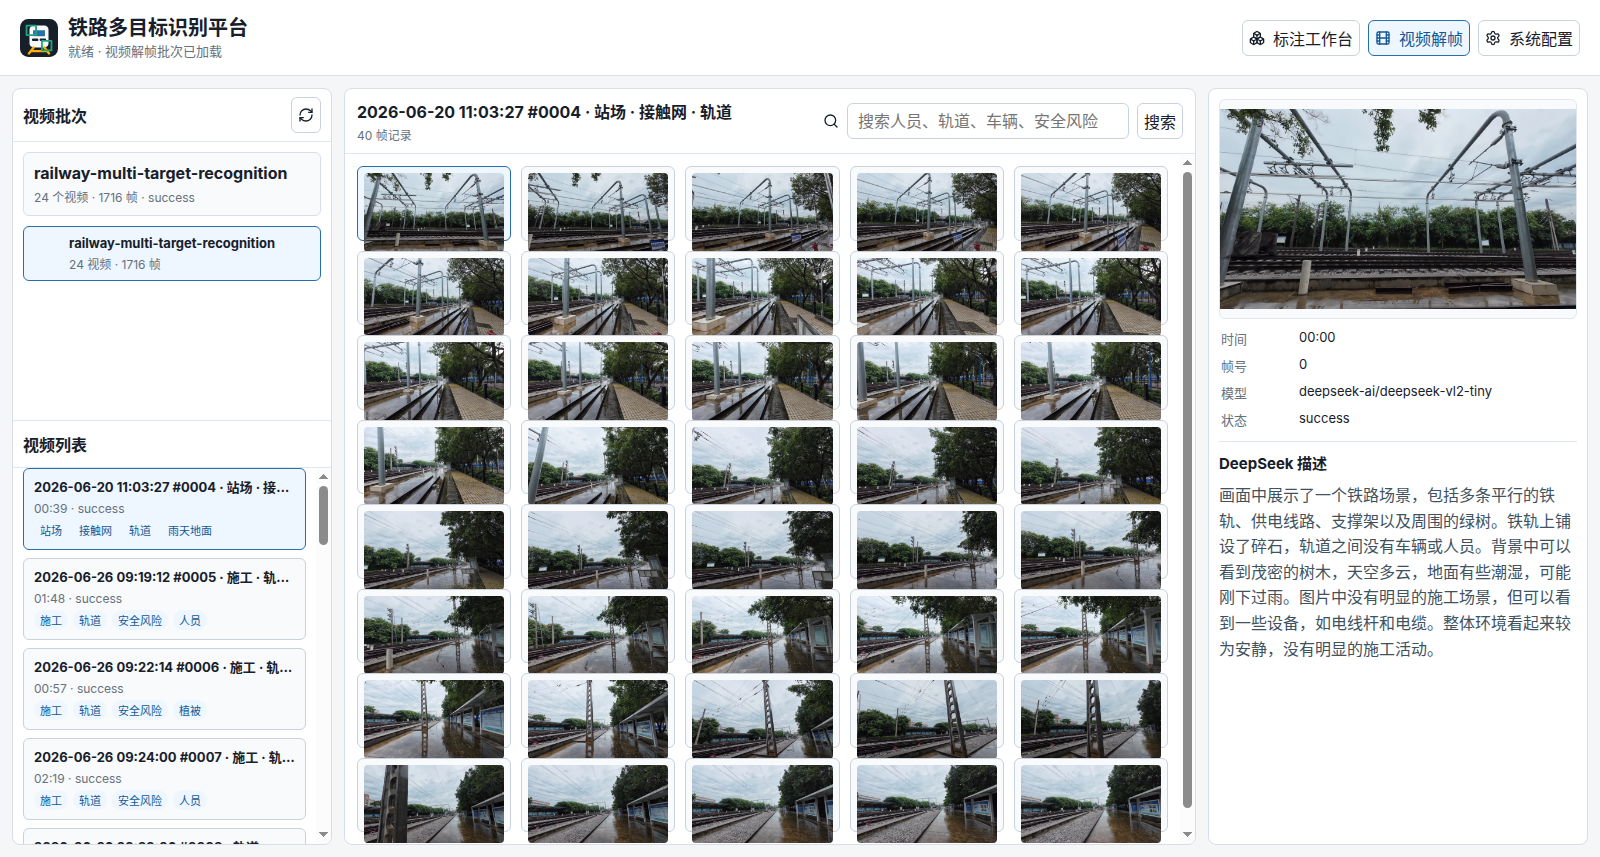
\includegraphics[width=0.96\textwidth]{figures/frontend_video_caption_page.png}
\caption{视频解帧与语义浏览前端界面\realmark}
\label{fig:frontend-screenshot}
\end{figure}

\subsection{原型验证与结果分析}

\subsubsection{数据与处理结果}

本文使用大疆无人机拍摄的真实巡检视频进行系统验证。系统共处理\keynum{24段视频}，并按约每秒一帧的策略生成\keynum{1716帧}图像描述记录。所有视频和帧记录均已入库，批次状态为 success。图\ref{fig:real-frames}展示了部分真实巡检帧，覆盖接触网、轨道扣件、现场作业和设备间等典型场景。表\ref{tab:result}给出了系统处理统计。

\begin{figure}[H]
\centering
\begin{minipage}{0.48\textwidth}
  \centering
  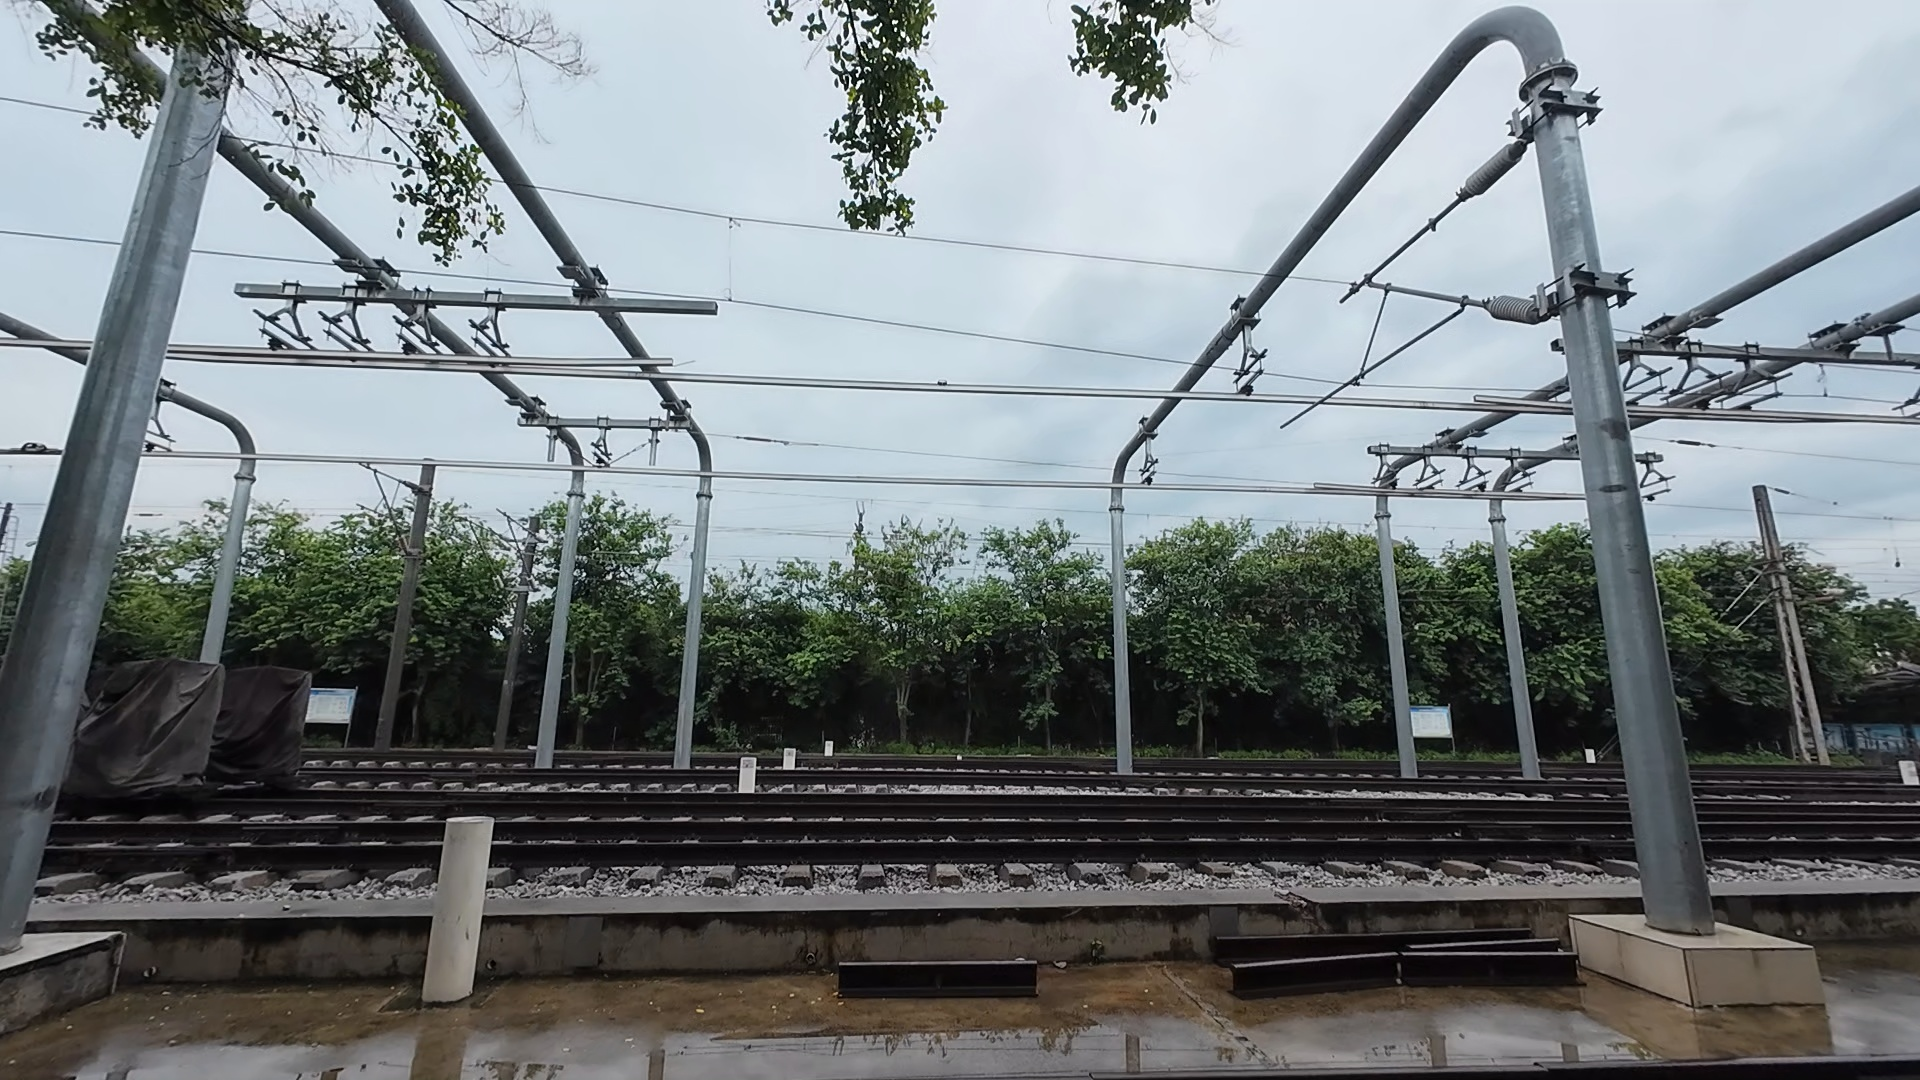
\includegraphics[width=\linewidth,height=35mm,keepaspectratio]{figures/sample_catenary_track.jpg}\\
  \small (a) 接触网与轨道场景
\end{minipage}
\hfill
\begin{minipage}{0.48\textwidth}
  \centering
  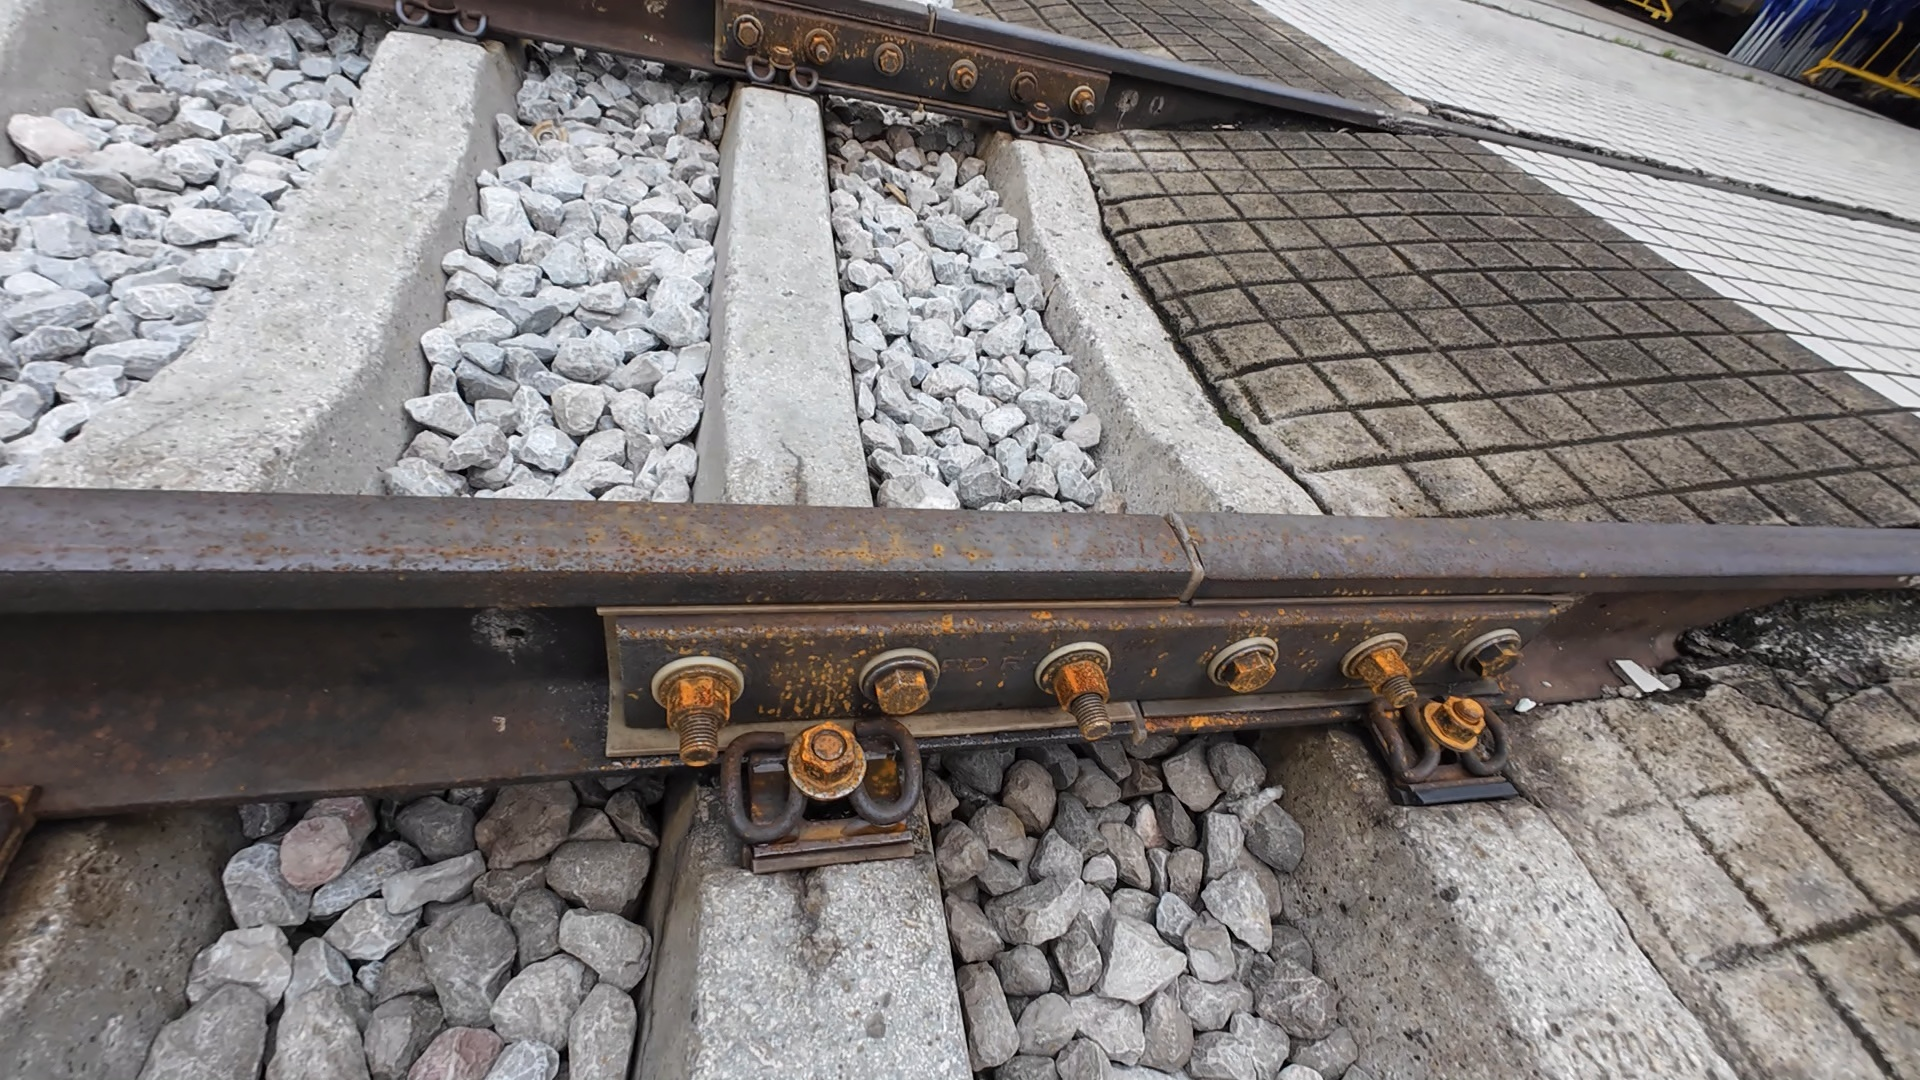
\includegraphics[width=\linewidth,height=35mm,keepaspectratio]{figures/sample_fastener.jpg}\\
  \small (b) 轨道扣件与道床
\end{minipage}

\vspace{0.6em}

\begin{minipage}{0.48\textwidth}
  \centering
  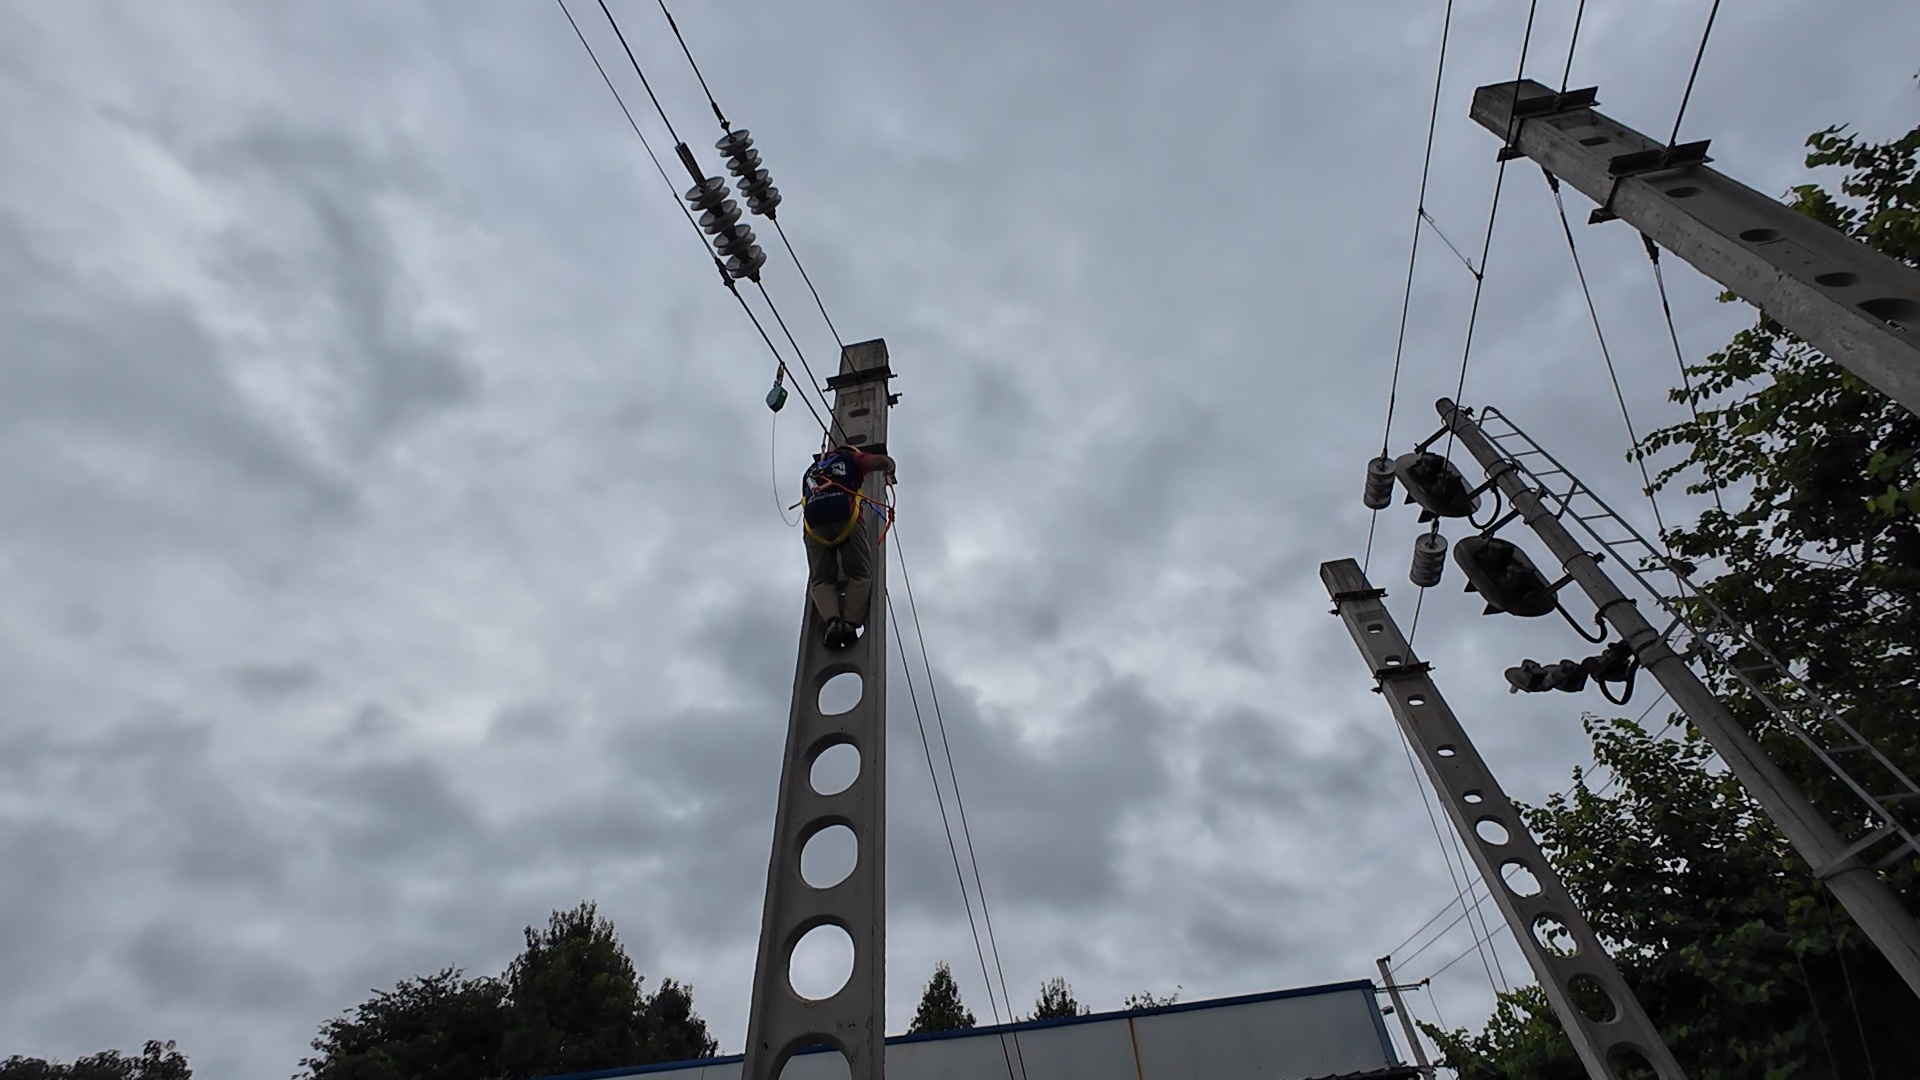
\includegraphics[width=\linewidth,height=35mm,keepaspectratio]{figures/sample_catenary_work.jpg}\\
  \small (c) 接触网作业与人员
\end{minipage}
\hfill
\begin{minipage}{0.48\textwidth}
  \centering
  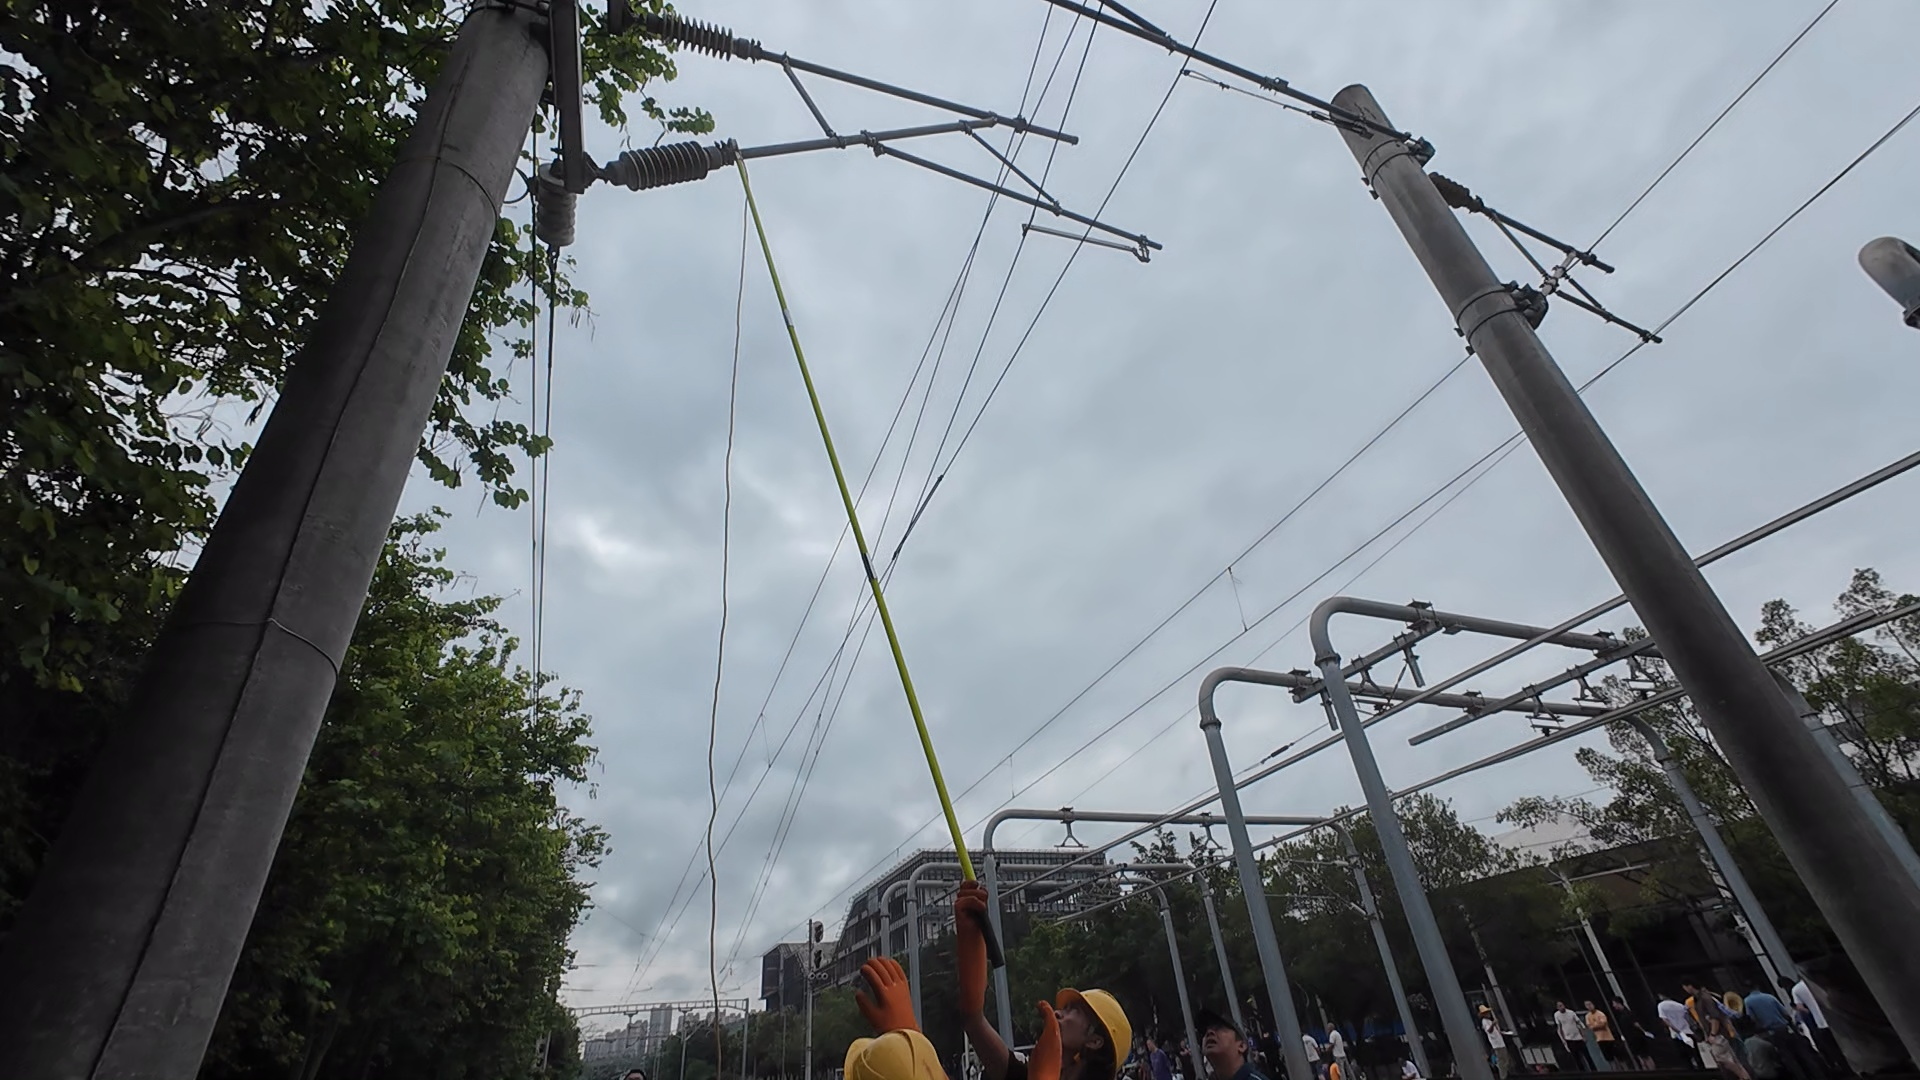
\includegraphics[width=\linewidth,height=35mm,keepaspectratio]{figures/sample_outdoor_catenary_inspection.jpg}\\
  \small (d) 户外接触网检测作业
\end{minipage}
\caption{真实铁路巡检视频抽帧样例\realmark}
\label{fig:real-frames}
\end{figure}

\begin{table}[H]
\centering
\caption{系统验证数据统计}
\label{tab:result}
\begin{tabularx}{0.86\textwidth}{>{\raggedright\arraybackslash}X r}
\toprule
指标 & 结果 \\
\midrule
视频批次名称 & railway-multi-target-recognition \\
视频数量 & \keynum{24} \\
抽帧数量 & \keynum{1716} \\
描述模型 & DeepSeek-VL2 \\
目标检测模型 & YOLO 系列 \\
关键词类别 & 接触网、轨道、人员、设备、施工、安全风险等 \\
数据库状态 & 全部入库成功 \\
前端展示 & 支持视频列表、帧浏览、关键词与描述查看 \\
\bottomrule
\end{tabularx}
\end{table}

\subsubsection{视频级语义命名结果}

为了使视频列表不再只显示日期型文件名，系统根据帧级描述自动提取关键词，并生成视频级展示名称。表\ref{tab:sample-videos}列出部分样例。

\begin{table}[H]
\centering
\caption{视频语义展示名称示例}
\label{tab:sample-videos}
\small
\begin{tabularx}{\textwidth}{>{\raggedright\arraybackslash\ttfamily\scriptsize}p{0.36\textwidth}>{\raggedright\arraybackslash\small}X}
\toprule
视频拍摄编号 & 语义展示名称 \\
\midrule
\shortstack[l]{20260620\_110327\\0004\_D.MP4} & 2026-06-20 11:03:27 \#0004 · 站场 · 接触网 · 轨道 \\
\shortstack[l]{20260626\_091912\\0005\_D.MP4} & 2026-06-26 09:19:12 \#0005 · 施工 · 轨道 · 安全风险 \\
\shortstack[l]{20260626\_093225\\0009\_D.MP4} & 2026-06-26 09:32:25 \#0009 · 施工 · 轨道 · 人员 \\
\shortstack[l]{20260626\_093407\\0011\_D.MP4} & 2026-06-26 09:34:07 \#0011 · 轨道 · 车辆 · 施工 \\
\shortstack[l]{20260626\_154839\\0024\_D.MP4} & 2026-06-26 15:48:39 \#0024 · 施工 · 设备 · 安全风险 \\
\bottomrule
\end{tabularx}
\end{table}

\subsubsection{结果分析}

验证结果表明，该系统能够将原始铁路巡检视频转化为中文结构化语义数据。与仅保存视频文件相比，结构化后的数据具有三个优势：第一，视频可以按关键词快速筛选，例如“接触网、人员、设备、安全风险”；第二，帧级描述保留了时间戳和图像路径，便于人工复核；第三，中文语义结果已经具备稳定的数据结构，可以作为后续建设双语术语映射和报告生成模块的输入基础。

同时，当前系统仍存在不足：关键词抽取以规则法为主，对复杂语义的泛化能力有限；双语和多语种服务仍处于架构预留阶段，需要补充术语库、翻译质量评估和人工审校机制；目标检测模型尚未针对东南亚铁路场景进行专门训练。后续工作将围绕铁路专用数据集构建、多语言术语库完善和风险分级模型展开。

\section{典型应用与量化价值}

\subsection{跨区域部署与应用前景}

面向马东铁及其他东南亚铁路场景，系统应支持现场边缘设备、中心数据库和远程专家协同部署。图\ref{fig:deploy}展示了跨区域部署架构。当前阶段由现场侧采集视频并完成抽帧和中文推理，中心侧保存结构化数据，通过 Web 平台提供中文结果浏览和人工复核；完成双语模块建设后，再向中方工程师、马来西亚本地运维人员和联合运维管理层提供经术语校验的双语结果。

\begin{figure}[H]
\centering
\begin{tikzpicture}
  \node[anchor=south west,inner sep=0] (depimg) at (0,0)
    {\includegraphics[width=0.96\textwidth]{04-edge-cloud-deployment.png}};
  \foreach \pos/\txt in {0.125/马东铁现场采集,0.385/边缘智能处理,0.68/中心数据与知识平台,0.905/中马协同应用} {
    \node[font=\scriptsize\bfseries,text width=30mm,align=center,yshift=-4.5mm]
      at ($(depimg.north west)!\pos!(depimg.north east)$) {\txt};
  }
\end{tikzpicture}
\caption{面向马东铁跨区域运维的边缘--中心协同架构}
\label{fig:deploy}
\end{figure}

该部署模式适用于带宽受限、人员分布分散和跨语言协作频繁的铁路建设与运维场景。当前先形成“现场采集、边缘处理、中心管理、中文复核”的稳定链路；未来再按项目需求接入术语库、语言接口和人工审校机制，在不影响现有巡检功能的前提下逐步提升跨语言协作能力。

\begin{figure}[H]
\centering
\includegraphics[width=0.86\textwidth]{07-international-multilingual-future.png}
\caption{面向东南亚铁路运维的国际化多语种协同应用构想}
\label{fig:multilingual-future}
\end{figure}

如图\ref{fig:multilingual-future}所示，国际化能力将作为现有中文风险识别系统的后续扩展，而不是当前功能。规划分三阶段实施：第一阶段建设中英铁路术语映射和双语报告模板；第二阶段补充马来语术语库、人工审校流程和联合运维角色权限；第三阶段根据东盟铁路项目需要扩展泰语、老挝语、越南语和印尼语，并形成“统一风险编码、分语种表达、人工确认后发布”的多语种知识服务。该路线既保持当前系统功能表述真实，也为跨区域培训、远程专家复核和本地化运维预留明确的演进空间。

\subsection{接触网试点案例与量化价值}

\subsubsection{试点案例设计}

本方案选择“接触网与线路环境视频巡检”作为首个试点，而不是一开始覆盖全部铁路专业。原因是现有数据已经包含接触网、轨道、人员和现场作业等高频对象，且无人机能够在不增加人员上线暴露的情况下快速形成连续视频证据。Network Rail 的公开实践表明，无人机可用于架空线路、结构物、排水、侵限和植被等巡检，并能减少不必要的轨旁人工检查\cite{networkrail-drones}。世界银行铁路资产管理研究也将视频、目视检查、探测设备和检测车辆列为资产状态数据来源，强调准确资产台账和持续更新的重要性\cite{worldbank-rail-asset}。这些案例说明“空中采集+结构化资产数据+人工复核”具备跨铁路项目的通用基础，但不能直接替代当地检修规程和专业人员判断。

试点范围建议选择一个边界清晰、便于复查的接触网工区，以月度或专项巡检任务为单位运行。系统按“任务建批次、视频自动解帧、模型生成描述、规则抽取风险、人工确认、导出记录”的闭环处理，典型业务设计见表\ref{tab:pilot-case}。

\begin{table}[H]
\centering
\caption{接触网巡检试点的业务闭环与验收证据}
\label{tab:pilot-case}
\small
\begin{tabularx}{\textwidth}{p{0.14\textwidth}p{0.23\textwidth}p{0.29\textwidth}X}
\toprule
环节 & 现场任务 & 系统处理 & 验收证据 \\
\midrule
任务准备 & 明确区段、日期、飞行和安全边界 & 建立批次、设备与人员标识 & 任务单、授权记录、批次编号 \\
数据采集 & 拍摄接触网、支柱、轨道和周界 & 校验文件、时间和来源元数据 & 原始视频哈希、采集日志 \\
智能处理 & 无需逐帧人工播放 & 自动抽帧、中文描述、关键词与风险提示 & 帧图、时间戳、模型版本、处理日志 \\
专业复核 & 工区人员确认对象与风险 & 修改标签、记录复核结论与责任人 & 复核前后版本、审计轨迹 \\
处置闭环 & 按既有规程决定复查或维修 & 关联处置状态，不自动下发安全指令 & 问题清单、复查图片、关闭时间 \\
复盘沉淀 & 周/月度分析典型问题 & 按区段、对象、风险类别聚合 & 月报、案例库、模型改进样本 \\
\bottomrule
\end{tabularx}
\end{table}

当前原型的可验证证据是\keynum{24段视频、1716帧记录、完整数据库链路和Web复核页面}；现场缺陷识别准确率、节省工时和闭环时长尚未经过马东铁真实生产试点验证。因此，表\ref{tab:pilot-kpi}中的数值定义为下一阶段验收目标，而不是本文已经取得的成效。

\begin{table}[H]
\centering
\caption{试点验收指标与测量方法}
\label{tab:pilot-kpi}
\small
\begin{tabularx}{\textwidth}{p{0.25\textwidth}p{0.18\textwidth}X p{0.18\textwidth}}
\toprule
指标 & 目标值 & 测量方法 & 责任方 \\
\midrule
视频处理成功率 & $\geq98\%$ & 成功任务数/有效任务数，失败任务可重试并留痕 & 平台实施方 \\
记录可追溯率 & $100\%$ & 抽查风险记录能否回溯原视频、帧、时间戳和模型版本 & 联合验收组 \\
高频对象准确率 & $\geq85\%$ & 专家标注盲测集上计算精确率，按对象分别报告 & 专业工区 \\
风险提示召回率 & $\geq90\%$ & 对试点确认风险计算召回率；未达标不得用于辅助放行 & 安全与技术组 \\
人工复核工时下降 & $\geq50\%$ & 同批视频采用原流程与系统辅助流程进行AB计时 & 运维管理方 \\
严重问题闭环率 & $100\%$ & 已确认严重问题均有责任人、处置状态与复查证据 & 业务负责人 \\
\bottomrule
\end{tabularx}
\end{table}

\subsubsection{可复制的典型场景组合}

在接触网试点稳定后，系统不通过重新建设平台复制，而是通过更换标签体系、规则模板和专业模型扩展场景。世界银行关于气候韧性交通的指导强调铁路运营维护应覆盖线路、电气化、车站、车辆和信息通信等子系统，并持续开展系统检查与状态监测\cite{worldbank-resilient-transport}。结合现有系统边界，可形成四类复制包：一是接触网与支柱状态巡检；二是轨道、扣件和道床表观巡检；三是施工人员、防护和线路侵限辅助检查；四是培训案例与远程专家复核。前两类面向设备运维，第三类面向安全管理，第四类面向知识沉淀，底层共享视频、帧、标签、版本与审计数据结构。

\subsubsection{投入产出情景测算}

投入产出采用“可核验成本+保守劳动节约”的口径，不把尚未验证的故障避免、停运损失或安全价值强行货币化。表\ref{tab:pilot-budget}给出一个工区级、4个月试点的人民币含税规划估算，实际金额需在现场调研和采购询价后确认。

\begin{table}[H]
\centering
\caption{工区级试点投入估算（规划值）}
\label{tab:pilot-budget}
\begin{tabularx}{0.88\textwidth}{>{\raggedright\arraybackslash}X r}
\toprule
投入项 & 估算金额（万元） \\
\midrule
边缘推理工作站与必要配件 & 4.5 \\
中心存储、备份与网络安全配置 & 2.0 \\
平台适配、接口集成与部署 & 7.0 \\
专业样本标注、规则与模型适配 & 3.0 \\
现场培训、试运行和验收支持 & 2.0 \\
风险准备金 & 2.5 \\
\midrule
\textbf{试点一次性投入合计} & \keynum{21.0} \\
预计年度运行维护 & 5.0 \\
\bottomrule
\end{tabularx}
\end{table}

假设试点转入常态后每年处理2000小时巡检视频，原流程平均需要1.0人工小时/视频小时，系统辅助后需要0.25人工小时/视频小时，综合人工成本按120元/小时计算，则年度直接工时节约为
\[
(1.0-0.25)\times 2000\times120={\color{railred}\mathbf{18}}\text{万元}
\]
即年度直接工时节约为\keynum{18万元}。扣除5万元年度运维后，保守年度净收益约13万元，静态回收期约为$21/13\times12={\color{railred}\mathbf{19.4}}\text{个月}$。这是用于验证商业可行性的情景测算，不是已实现收益；正式项目应以试点AB计时、当地人工成本、视频规模和采购价格重新计算。风险早发现、减少人员上线、缩短问题检索时间等价值单独作为安全与管理指标衡量，避免重复计价。

\section{落地实施与商业推广}

\subsection{分阶段实施路径}

实施遵循“先基线、后试点；先辅助、后扩展；每阶段可验收、不可越级”的原则。资产管理体系建设应把性能、风险和支出纳入统一决策，这与ISO 55001:2024强调的资产管理目标、决策与持续改进要求一致\cite{iso55001}。项目计划见表\ref{tab:implementation-plan}。

\begin{table}[H]
\centering
\caption{项目实施里程碑与退出条件}
\label{tab:implementation-plan}
\small
\begin{tabularx}{\textwidth}{p{0.12\textwidth}p{0.14\textwidth}p{0.30\textwidth}X}
\toprule
阶段 & 周期 & 主要工作与交付物 & 阶段门禁 \\
\midrule
0 基线调研 & 第1--2周 & 业务流程、资产字典、数据清单、飞行合规、网络与安全边界 & 试点区段、责任人、基线指标获书面确认 \\
1 环境部署 & 第3--4周 & 本地服务器、PostgreSQL、对象存储、账号权限、备份与监控 & 安全检查通过，原始数据可回滚 \\
2 数据适配 & 第5--8周 & 样本清洗、专业标注、标签字典、模型和规则适配 & 金标集冻结，关键对象指标达到内部测试线 \\
3 业务试运行 & 第9--12周 & 真实任务并行运行、人工复核、问题闭环、AB工时记录 & 不影响原安全流程，重大缺陷零漏处置 \\
4 验收优化 & 第13--16周 & KPI复测、用户培训、运维手册、验收报告 & 表\ref{tab:pilot-kpi}逐项签字，不合格项限期整改 \\
5 复制推广 & 第5--12月 & 扩区段、扩专业、接口标准化和多语种术语准备 & 单工区稳定运行不少于3个月后再复制 \\
\bottomrule
\end{tabularx}
\end{table}

实施组织采用联合项目组：业主或运维单位担任业务负责人并批准安全边界；接触网、工务和安全专业人员负责金标集与问题定级；平台团队负责部署、模型、数据和故障响应；信息安全人员负责账号、日志、备份和漏洞处置；当地培训骨干负责用户培训与术语反馈。MRL公开资料显示，首批66名赴华培训人员已于2026年完成培训并进入ECRL运营维护相关岗位，且自2025年5月起已有259名马来西亚学员参与相关培训\cite{mrl-training-2026}，这为建立“当地专业人员复核+中方专家远程支持”的试点组织提供了现实人才基础。

\subsection{软硬件与运行保障}

试点优先复用现有视频拍摄设备，不将新购无人机作为系统落地前提。边缘侧建议配置一台24GB级显存的推理工作站，用于离线批处理；中心侧建议不少于8核CPU、32GB内存和2TB可扩展存储，并配置独立备份。软件侧继续采用Web前端、API服务、PostgreSQL、任务队列和模型适配层，所有模型输出保存模型版本、阈值和原始证据。断网时允许现场采集与本地暂存，恢复连接后再同步；平台故障时回退到原人工流程，任何时候均不因AI不可用而阻断既有安全作业。

项目建立三级响应机制：影响浏览的普通问题在1个工作日内响应；影响批处理的高优问题在4小时内响应；涉及数据泄露、错误高风险提示或系统性漏检的严重事件立即停用相关模型版本，保留证据并启动人工复查。上线后的月度运行报告至少包含任务成功率、复核量、误报漏报、数据增长、故障时长和改进项。

\subsection{商业模式与推广路径}

\subsubsection{目标客户与产品组合}

目标客户不是普通视频用户，而是铁路基础设施业主、运营维护合资公司、工程承包商、专业检修单位和铁路培训机构。商业产品采用“平台底座+专业场景包+实施服务”的组合：平台底座提供数据、任务、权限、审计和前端复核；场景包提供接触网、轨道或施工安全标签与规则；实施服务负责私有部署、系统集成、样本适配和培训。未来多语种知识服务必须在术语库和人工审校成熟后作为独立增值模块提供，不计入当前产品功能。

\begin{table}[H]
\centering
\caption{商业产品层级与适用客户（规划）}
\label{tab:commercial-packages}
\small
\begin{tabularx}{\textwidth}{p{0.18\textwidth}p{0.22\textwidth}p{0.24\textwidth}X}
\toprule
产品层级 & 典型客户 & 交付内容 & 收费与价值验证 \\
\midrule
验证试点包 & 单一工区、工程项目部 & 1个场景、4个月试点、培训与验收 & 规划价20--30万元；先证明数据闭环与工时节约 \\
私有部署版 & 运营公司、基础设施业主 & 本地平台、接口、权限审计、2--3个场景包 & 规划价50--120万元；按规模和集成范围询价 \\
年度技术服务 & 已部署客户 & 升级、监控、规则和模型维护、季度复盘 & 原交付额的15\%--20\%/年或按服务级别定价 \\
专业知识服务 & 培训机构、跨国运维团队 & 案例库、术语库与未来多语种审核流程 & 后续模块；完成真实验证后单独定价 \\
\bottomrule
\end{tabularx}
\end{table}

表中价格仅是参赛方案的商业规划区间，不构成市场报价。早期收入以实施和私有部署为主，随着接口、标签和场景包标准化，逐步提高可复用软件许可与年度服务比例。数据所有权归客户，平台不通过转售巡检视频获利，模型改进数据的使用范围由合同明确。

\subsubsection{从马东铁到东南亚的复制路径}

推广采用“三步走”。第一步，在马东铁单工区完成中文巡检闭环和量化验收，形成经过客户确认的基线、案例和部署手册；第二步，复制到同一线路其他工区及培训场景，验证跨专业标签和组织协同；第三步，通过当地铁路培训机构、工程总承包与运维合作伙伴进入其他东盟铁路项目。ASEAN Digital Masterplan 2030提出通过培训、共享数字能力、同伴学习和技术援助缩小互操作、数据治理与AI治理能力差距\cite{asean-digital-2030}，本方案的推广重点因此应是可移交的数据规范、运维流程和本地人才能力，而不是单纯输出模型。

每次复制保留统一的任务、证据、审计和接口标准，同时允许当地修改资产字典、风险等级、语言和审批流程。复制项目必须重新完成现场基线、法规审查和金标集测试；不得把马东铁试点指标直接视为其他国家项目的性能承诺。渠道上优先与铁路业主、联合运维公司、铁路院校和具备飞行资质的本地服务商合作，以联合交付降低进入成本和售后半径。

\subsubsection{竞争壁垒与持续经营}

方案的竞争力不依赖单一视觉模型，而来自四项可积累资产：一是带时间戳和复核版本的铁路视频数据结构；二是由专业人员确认的场景金标集；三是面向接触网、轨道和施工安全的术语与规则包；四是可私有部署、可更换模型的工程平台。持续经营指标包括试点转正式部署率、年度续约率、单场景交付周期、有效复核样本增长和客户问题闭环时长。任何商业材料均区分“原型已实现、试点目标、未来规划”，避免以未验证准确率或多语种能力进行销售承诺。

\section{风险保障与结论展望}

\subsection{风险管理与保障机制}

铁路属于安全关键基础设施，AI输出只能作为风险筛查和证据组织工具，最终判断由授权专业人员作出。风险治理参考NIST AI RMF的“治理、映射、测量、管理”闭环\cite{nist-ai-rmf}，网络安全参考NIST CSF 2.0的治理、识别、保护、检测、响应和恢复思路\cite{nist-csf}。主要风险与控制措施见表\ref{tab:risk-register}。

\begin{longtable}{p{0.16\textwidth}p{0.10\textwidth}p{0.28\textwidth}p{0.30\textwidth}}
\caption{项目风险登记册与控制措施}\label{tab:risk-register}\\
\toprule
风险 & 等级 & 触发信号与影响 & 预防、响应与责任人 \\
\midrule
\endfirsthead
\toprule
风险 & 等级 & 触发信号与影响 & 预防、响应与责任人 \\
\midrule
\endhead
模型漏检或误报 & 高 & 金标集召回下降、严重对象未提示；可能造成错误判断 & AI不自动放行或下工单；双人复核高风险项；版本回滚；专业负责人签字 \\
场景与数据漂移 & 高 & 季节、线路或设备变化导致指标持续下降 & 分区统计、月度抽检、漂移告警、增量标注；模型负责人维护 \\
飞行与现场安全 & 高 & 未取得许可、侵入限制空域或影响作业 & 仅由授权人员操作；任务前审批、地理围栏和现场隔离；安全负责人停止任务 \\
数据与隐私合规 & 高 & 视频出现可识别人员、跨境传输或超期保存 & 最小化采集、脱敏、本地存储、期限删除、访问审计；数据保护负责人审批 \\
网络与账号攻击 & 高 & 异常登录、批量下载、日志中断或勒索事件 & 最小权限、强认证、传输与存储加密、离线备份、演练恢复；安全管理员响应 \\
多语种术语偏差 & 中 & 同一风险在不同语言中等级或含义不一致 & 统一风险编码、双人术语审校、版本冻结；未验收语种不得用于正式报告 \\
用户采纳不足 & 中 & 复核积压、绕开系统、反馈质量下降 & 岗位培训、试点共创、保留原流程、按月复盘；业务负责人改进 \\
供应商或模型锁定 & 中 & 模型停更、许可变化、推理成本上升 & 模型适配层、开放数据导出、可替换推理后端；技术负责人准备替代方案 \\
进度与预算超支 & 中 & 里程碑延期超过2周或成本偏差超过10\% & 分阶段采购、范围冻结、风险准备金、门禁评审；项目经理纠偏 \\
商业回报不足 & 中 & 工时下降未达目标、试点无续约意向 & 用AB计时复核价值；缩小场景或停止扩张；商务与业主共同决策 \\
\bottomrule
\end{longtable}

无人机在马来西亚开展航空作业须遵守CAAM关于UAS授权、空域、高度、目视范围和人员安全的要求，标准授权通常需提前至少14个工作日提交材料\cite{caam-uas}。涉及可识别人员的视频及商业数据处理，还应结合马来西亚《个人数据保护法》及其数据泄露通知、数据保护官、跨境传输等配套指南开展影响评估\cite{malaysia-pdpa}。因此，进入马东铁现场前必须由当地法律、安全和数据负责人完成合规确认；本文不以技术方案替代飞行许可、铁路安全规程或法律意见。

项目设置明确的停用条件：连续两次验收未达到严重风险召回要求；发生未经授权的数据外传；模型版本不可追溯；或现场负责人认为系统影响安全作业。触发后立即切回人工流程，冻结相关数据和日志，完成原因分析、整改与重新验收后方可恢复。通过把“可停用、可回退、可审计”纳入设计，降低技术试点向生产系统迁移时的系统性风险。

\subsection{结论与展望}

本文提出一种面向东南亚铁路运维的多模态智能巡检与风险识别系统。当前原型围绕真实铁路巡检视频，完成了视频解帧、中文多模态识别、语义描述、关键词抽取、数据库管理和前端人工复核链路。基于\keynum{24段}巡检视频和\keynum{1716帧}图像的验证表明，系统已经能够生成可检索、可复核的中文结构化巡检记录，并为后续跨语言共享提供统一数据基础。

未来工作将从五个方向展开：第一，以马东铁典型岗位和设备体系为切入点，构建更大规模的东南亚铁路巡检数据集；第二，引入铁路专用目标检测和多标签风险识别模型；第三，优先完善中英双语及马来语术语库，再扩展泰语、老挝语、越南语和印尼语；第四，加入人工审核与主动学习闭环；第五，支持移动端采集和边缘部署，使系统能够更好地服务东南亚铁路长期运维。

\clearpage
\phantomsection
\addcontentsline{toc}{section}{参考文献}
\begin{thebibliography}{99}
\bibitem{mot-ecrl-overview} Ministry of Transport Malaysia. East Coast Rail Link (ECRL) 项目概况[EB/OL]. \href{https://www.mot.gov.my/my/land/development/ongoing-rail-project}{马来西亚交通部项目网页}, 访问日期：2026-07-21.
\bibitem{mot-ecrl-progress-2026} Ministry of Transport Malaysia. Siaran Media Kementerian Pengangkutan, 11 February 2026[EB/OL]. \href{https://www.mot.gov.my/en/Kenyataan\%20Media/Year\%202026/SIARAN\%20MEDIA\%20KEMENTERIAN\%20PENGANGKUTAN\%20\%28110226\%29\%20\%28v4\%29.pdf}{马来西亚交通部官方PDF}, 2026-02-11.
\bibitem{ecrl-joint-operation} 新华社“一带一路”网. 中马签署协议成立马东铁运营维护合资公司[EB/OL]. \href{https://www.yidaiyilu.gov.cn/p/0P55S56C.html}{报道网页}, 2024-12-19.
\bibitem{ndrc-ecrl-training} National Development and Reform Commission. China-Malaysia railway training cooperation supports ECRL talent development[EB/OL]. \href{https://en.ndrc.gov.cn/netcoo/achievements/202207/t20220728_1332745.html}{国家发展改革委英文网页}, 2022-07-28.
\bibitem{mot-plki-2025} Ministry of Transport Malaysia. Teks Ucapan Program Latihan Kemahiran Industri ECRL bagi Fasa Operasi dan Penyelenggaraan[EB/OL]. \href{https://www.mot.gov.my/my/Ucapan\%20YBM/Tahun\%202025/Teks\%20Ucapan\%20YB\%20MOT\%20-\%20PLKI-ECRL\%20O\%26M.pdf}{马来西亚交通部官方PDF}, 2025.
\bibitem{china-malaysia-joint-statement} Ministry of Foreign Affairs Malaysia. Joint Statement Between the People's Republic of China and Malaysia on Building a High-level Strategic Malaysia-China Community with a Shared Future[EB/OL]. \href{https://www.kln.gov.my/web/guest/-/joint-statement-between-the-people-s-republic-of-china-and-malaysia-on-building-a-high-level-strategic-malaysia-china-community-with-a-shared-future-1}{马来西亚外交部联合声明}, 2025-04-17.
\bibitem{asean-china-action-plan} 中华人民共和国外交部. 中国--东盟全面战略伙伴关系行动计划（2026--2030）[EB/OL]. \href{https://www.mfa.gov.cn/wjbzhd/202508/P020250829826265881620.pdf}{中国外交部官方PDF}, 2025.
\bibitem{asean-rail-training} 新华社“一带一路”网. 东盟国家轨道交通标准及运营管理研修班在华举办[EB/OL]. \href{https://www.yidaiyilu.gov.cn/p/05CAJT2H.html}{报道网页}, 访问日期：2026-07-21.
\bibitem{yolo} Redmon J., Divvala S., Girshick R., Farhadi A. You Only Look Once: Unified, Real-Time Object Detection[C]//CVPR. 2016: 779--788.
\bibitem{clip} Radford A., Kim J. W., Hallacy C., et al. Learning Transferable Visual Models From Natural Language Supervision[C]//ICML. 2021: 8748--8763.
\bibitem{blip} Li J., Li D., Xiong C., Hoi S. BLIP: Bootstrapping Language-Image Pre-training for Unified Vision-Language Understanding and Generation[C]//ICML. 2022: 12888--12900.
\bibitem{deepseekvl} DeepSeek-AI. DeepSeek-VL2: Mixture-of-Experts Vision-Language Models for Advanced Multimodal Understanding[EB/OL]. \href{https://github.com/deepseek-ai/DeepSeek-VL2}{项目仓库}, 2024.
\bibitem{networkrail-drones} Network Rail. Drones or Unmanned Aircraft Systems: How We Use Drones[EB/OL]. \href{https://www.networkrail.co.uk/our-work/looking-after-the-railway/our-fleet-machines-and-vehicles/air-operations/drones-or-unmanned-aircraft-systems-uas/}{Network Rail官方网站}, 访问日期：2026-07-22.
\bibitem{worldbank-rail-asset} World Bank. Serbia Railways Asset Management Plan Using Life-Cycle Costs[R/OL]. \href{https://documents1.worldbank.org/curated/en/726091593064265592/pdf/Serbia-Railways-Asset-Management-Plan-Using-Life-Cycle-Costs.pdf}{世界银行报告}, 2020.
\bibitem{worldbank-resilient-transport} World Bank. Disaster and Climate-Resilient Transport Guidance Note[R/OL]. \href{https://documents1.worldbank.org/curated/en/099032625173042760/pdf/P180423-670950ea-9b3e-4cb2-a416-bf19ee625e3e.pdf}{世界银行报告}, 2026.
\bibitem{iso55001} International Organization for Standardization. ISO 55001:2024 Asset Management---Asset Management System---Requirements[S/OL]. \href{https://www.iso.org/standard/83054.html}{ISO官方网站}, 2024.
\bibitem{mrl-training-2026} Malaysia Rail Link. 66 Pelatih Malaysia Tamat Latihan Rel di China, Bakal Terajui Operasi ECRL[EB/OL]. \href{https://www.mrl.com.my/my/66-pelatih-malaysia-tamat-latihan-rel-di-china-bakal-terajui-operasi-ecrl/}{MRL官方网站}, 2026-05-21.
\bibitem{asean-digital-2030} Association of Southeast Asian Nations. ASEAN Digital Masterplan 2030[R/OL]. \href{https://asean.org/wp-content/uploads/2026/01/ASEAN-Digital-Master-Plan-2030-final-2026.pdf}{ASEAN官方网站}, 2026.
\bibitem{nist-ai-rmf} Tabassi E. Artificial Intelligence Risk Management Framework (AI RMF 1.0)[R/OL]. \href{https://doi.org/10.6028/NIST.AI.100-1}{NIST AI 100-1}, 2023.
\bibitem{nist-csf} National Institute of Standards and Technology. The NIST Cybersecurity Framework (CSF) 2.0[R/OL]. \href{https://www.nist.gov/cyberframework}{NIST官方网站}, 2024.
\bibitem{caam-uas} Civil Aviation Authority of Malaysia. Unmanned Aircraft System (UAS): Regulations and Standard Authorisation to Fly[EB/OL]. \href{https://www.caam.gov.my/public/unmanned-aircraft-system-uas/}{CAAM官方网站}, 访问日期：2026-07-22.
\bibitem{malaysia-pdpa} Personal Data Protection Commissioner Malaysia. Personal Data Protection Act 2010 [Act 709] and Related Guidelines[EB/OL]. \href{https://www.pdp.gov.my/ppdpv1/en/akta/pdp-act-2010-en/}{马来西亚个人数据保护局官方网站}, 访问日期：2026-07-22.
\end{thebibliography}

\end{document}
